\section{Results}\label{sec:results}
All numbers below were measured on data the models never trained on (Section~\ref{sec:data}); where a caveat applies it is stated next to the number.

\subsection{Naming the pose from one frame}
\textbf{Progress over model generations.} Table~\ref{tab:posehead} follows the pose model from the first (about two-month-old) model to the current one. On the held-out public photos the earliest models passed no pose; the current gate model passes three with 22.6\% false alarms. The 86--90\% that two September models score on all 422 Commons photos is deliberately omitted because they were trained on most of those photos.
\begin{table}[t]
\centering\footnotesize
\caption{Pose-head generations on clean tests. Frozen Commons-103: none of these models trained on those photos (the new model is scored out-of-fold). Held-out public photos: 1{,}685 (1{,}037 other poses); $v4$ may have seen similar public images, which can only flatter it.}\label{tab:posehead}
\begin{tabular}{@{}lrrrr@{}}
\toprule
 & \multicolumn{2}{c}{Frozen Commons-103} & \multicolumn{2}{c}{Held-out public} \\
Model & Overall & Macro rec. & Poses pass & False alarm \\ \midrule
19 Jul original & 23.3\% & 17.5\% & 0 & 75.0\% \\
3 Sep retrain & 13.6\% & 11.1\% & 0 & 64.5\% \\
21 Sep $v4$ (was live) & \textbf{60.2\%} & \textbf{64.8\%} & 1 & 81.5\% \\
New (gate model) & 49.5\% & 58.0\% & \textbf{3} & \textbf{22.6\%} \\ \bottomrule
\end{tabular}
\end{table}

\textbf{The decision path matters more than the model.} Table~\ref{tab:policy} and Fig.~\ref{fig:charts}a compare decision policies on the 1{,}685 held-out public photos using the real production functions. Through the original path (rule engine wins every disagreement) a new MLP changed nothing: identical to rules-only (36.9\%, 78.3\% false alarms, no pose passing). The cascade reaches 78.9\% with 20.8\% false alarms and seven poses at recall and precision $\ge0.70$ (chair, corpse, downward dog, tree, triangle, upward dog, Warrior~II). The policy was chosen on a validation half only (79.3\%, 20.1\%, 3 poses) and confirmed on the untouched half (78.6\%, 21.6\%, 4 poses: corpse, downward dog, tree, Warrior~II). On the wild frozen-103 set the cascade scores 55.3\% against 37.9--40.8\% before; $v4$ alone is better at pure naming there (60.2\%), so the cascade gives up about five photos of naming accuracy for about 60 points fewer false alarms elsewhere. Through the real \texttt{/analyse\_frame} endpoint with the real models, switching the cascade off reproduced production exactly and switching it on reproduced 78.9\%/20.8\%/7, agreeing with the offline policy on 100\% of requests; a replay against the live Space gave 78.1\%/21.8\%/7 (16 of 1{,}685 requests were rejected by the host's rate limiter under an 8-thread stress test).
\begin{table}[t]
\centering\footnotesize\setlength{\tabcolsep}{4pt}
\caption{Decision policies on the 1{,}685 held-out public photos. False alarm: a photo of another pose named as one of ours (lower is better).}\label{tab:policy}
\begin{tabular}{@{}lrrr@{}}
\toprule
Policy & Overall & False alarm & Poses pass \\ \midrule
Production before ($v4$ + rules) & 36.9\% & 78.3\% & 0 \\
New model + rules & 36.9\% & 78.3\% & 0 \\
Rules only & 36.9\% & 78.3\% & 0 \\
$v4$ alone & 42.9\% & 81.5\% & 1 \\
Average of both MLPs & 65.2\% & 47.7\% & 5 \\
Veto lifted when rules agree & 65.9\% & 42.3\% & 5 \\
\textbf{Cascade} ($v4$ names, new model vetoes) & \textbf{78.9\%} & \textbf{20.8\%} & \textbf{7} \\ \bottomrule
\end{tabular}
\end{table}

\begin{figure*}[t]
\centering
\begin{subfigure}[t]{0.32\textwidth}\centering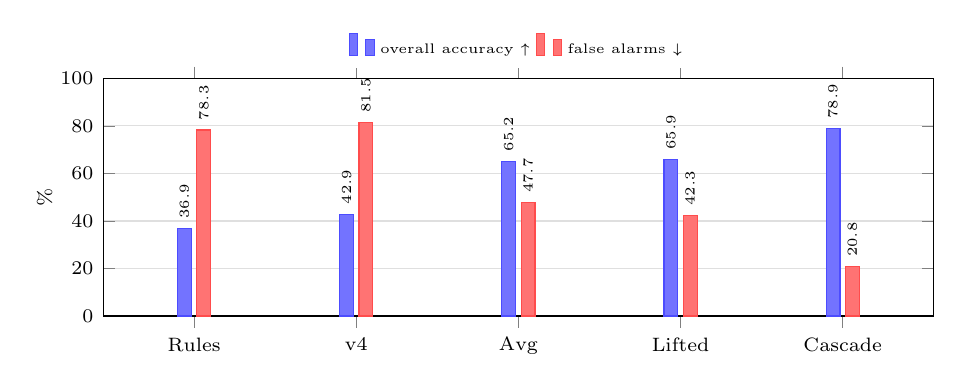
\begin{tikzpicture}
\begin{axis}[ybar,bar width=5pt,width=\linewidth,height=4.6cm,ymin=0,ymax=100,ylabel={\%},ylabel style={font=\scriptsize,yshift=-4pt},
  symbolic x coords={Rules,v4,Avg,Lifted,Cascade},xtick=data,x tick label style={font=\scriptsize},y tick label style={font=\scriptsize},
  legend style={font=\tiny,at={(0.5,1.04)},anchor=south,legend columns=2,draw=none},enlarge x limits=0.14,ymajorgrids,grid style={gray!25},
  nodes near coords,nodes near coords style={font=\tiny,/pgf/number format/fixed,/pgf/number format/precision=1},every node near coord/.append style={rotate=90,anchor=west}]
\addplot[fill=blue!55,draw=blue!70] coordinates {(Rules,36.9)(v4,42.9)(Avg,65.2)(Lifted,65.9)(Cascade,78.9)};
\addplot[fill=red!55,draw=red!70] coordinates {(Rules,78.3)(v4,81.5)(Avg,47.7)(Lifted,42.3)(Cascade,20.8)};
\legend{overall accuracy $\uparrow$,false alarms $\downarrow$}
\end{axis}
\end{tikzpicture}
\caption{Decision policies (held-out public photos)}\end{subfigure}\hfill
\begin{subfigure}[t]{0.32\textwidth}\centering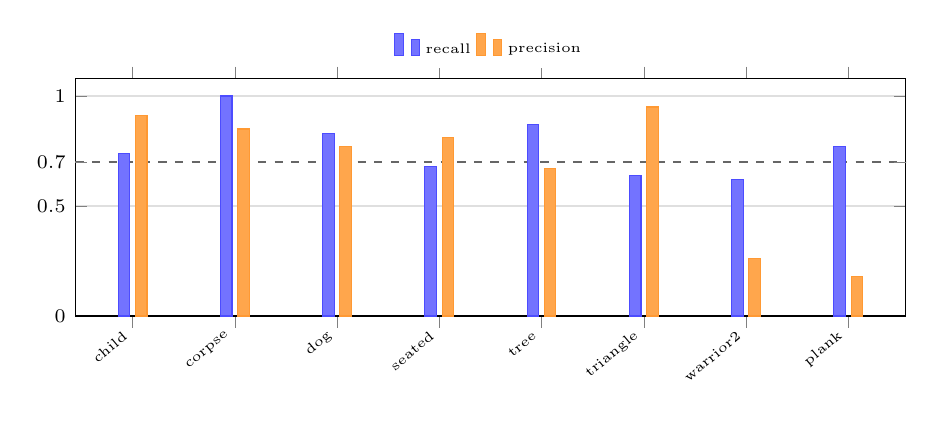
\begin{tikzpicture}
\begin{axis}[ybar,bar width=4.2pt,width=\linewidth,height=4.6cm,ymin=0,ymax=1.08,
  symbolic x coords={child,corpse,dog,seated,tree,triangle,warrior2,plank},xtick=data,x tick label style={font=\tiny,rotate=40,anchor=east},y tick label style={font=\scriptsize},
  legend style={font=\tiny,at={(0.5,1.04)},anchor=south,legend columns=2,draw=none},enlarge x limits=0.08,ymajorgrids,grid style={gray!25},
  extra y ticks={0.7},extra y tick style={grid=major,grid style={dashed,black!60},tick label style={font=\tiny}}]
\addplot[fill=blue!55,draw=blue!70] coordinates {(child,0.74)(corpse,1.00)(dog,0.83)(seated,0.68)(tree,0.87)(triangle,0.64)(warrior2,0.62)(plank,0.77)};
\addplot[fill=orange!70,draw=orange!80] coordinates {(child,0.91)(corpse,0.85)(dog,0.77)(seated,0.81)(tree,0.67)(triangle,0.95)(warrior2,0.26)(plank,0.18)};
\legend{recall,precision}
\end{axis}
\end{tikzpicture}
\caption{ST-GCN, held-out videos, per pose}\end{subfigure}\hfill
\begin{subfigure}[t]{0.32\textwidth}\centering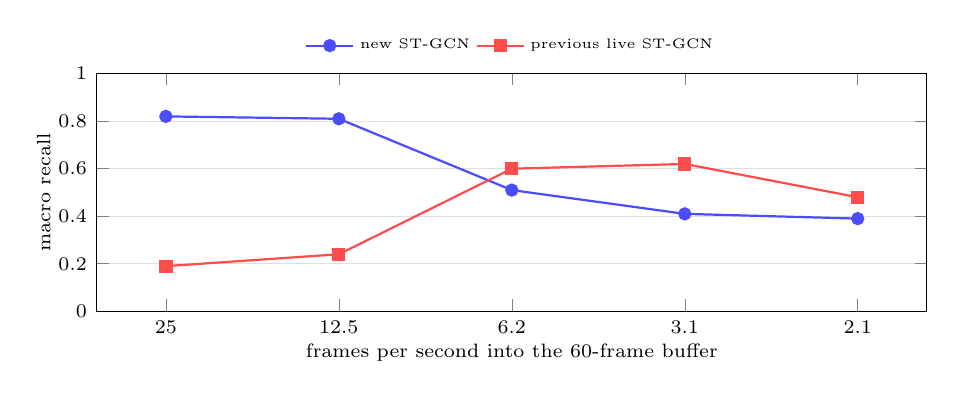
\begin{tikzpicture}
\begin{axis}[width=\linewidth,height=4.6cm,ymin=0,ymax=1,symbolic x coords={25,12.5,6.2,3.1,2.1},xtick=data,x tick label style={font=\scriptsize},y tick label style={font=\scriptsize},
  xlabel={frames per second into the 60-frame buffer},xlabel style={font=\scriptsize,yshift=3pt},ylabel={macro recall},ylabel style={font=\scriptsize,yshift=-4pt},
  legend style={font=\tiny,at={(0.5,1.04)},anchor=south,legend columns=2,draw=none},ymajorgrids,grid style={gray!25},enlarge x limits=0.1]
\addplot[blue!70,mark=*,thick] coordinates {(25,0.82)(12.5,0.81)(6.2,0.51)(3.1,0.41)(2.1,0.39)};
\addplot[red!70,mark=square*,thick] coordinates {(25,0.19)(12.5,0.24)(6.2,0.60)(3.1,0.62)(2.1,0.48)};
\legend{new ST-GCN,previous live ST-GCN}
\end{axis}
\end{tikzpicture}
\caption{ST-GCN input-rate contract}\end{subfigure}
\caption{(a)~Rules-only, $v4$, the average of both MLPs, the veto lifted when rules agree, and the cascade. (b)~Per-pose recall and precision of the final ST-GCN on videos it never trained on (dashed: 0.70 bar; warrior~2 and plank have few held-out windows). (c)~Macro recall on held-out videos when the 60-frame buffer is filled at different rates; the new model needs training-rate windows, the previous model was partly trained on slow windows.}
\label{fig:charts}
\end{figure*}

\subsection{Baselines: is the neural network necessary?}\label{sec:baselines}
To answer ``compared with what?'' we trained standard methods on exactly the rows the new MLP was trained on (136{,}506 rows of 15 zero-$z$ angles: cue-verified video frames, training photos and photos of other poses labelled transition/unknown) and scored them on the same photos with the same metrics: $k$-NN ($k{=}15$, distance-weighted), an RBF SVM, logistic regression, a 300-tree random forest, and a plain MLP (256--256--128, ReLU, no residual blocks or batch normalisation). The SVM, forest and logistic regression use class-balanced weights; the SVM sees at most 20{,}000 class-balanced rows, the other methods between 64{,}000 and 115{,}000. These runs use one random seed and were executed on Kaggle. Table~\ref{tab:baseline} and Fig.~\ref{fig:baseline} report two held-out sets: the 1{,}685 public photos (same public datasets as the training photos, disjoint files) and the frozen \emph{wild} Commons-103 photos from another source, scored out-of-fold.
\begin{table}[t]
\centering\footnotesize\setlength{\tabcolsep}{3.5pt}
\caption{Standard methods on the same data and held-out photos. Public: 1{,}685 held-out photos (1{,}037 other poses). Wild: frozen Commons-103, out-of-fold (a different source; with 103 photos, gaps under $\sim$10 points are within noise). $^\dagger$first of two runs.}\label{tab:baseline}
\begin{tabular}{@{}lrrrr@{}}
\toprule
 & \multicolumn{3}{c}{Public held-out} & Wild \\
Method & Overall & False alarm & Poses pass & Overall \\ \midrule
Production before ($v4$ + rules) & 36.9\% & 78.3\% & 0 & 37.9\% \\
Logistic regression$^\dagger$ & 29.7\% & 95.8\% & 1 & -- \\
$k$-NN & 58.6\% & 55.7\% & 1 & 50.5\% \\
SVM (RBF) & 58.4\% & 56.2\% & 3 & 52.4\% \\
Plain MLP & 80.9\% & 19.1\% & 3 & 47.6\% \\
Random forest & \textbf{85.3\%} & \textbf{9.8\%} & 7 & 35.0\% \\
$v4$ alone & 42.9\% & 81.5\% & 1 & \textbf{60.2\%} \\
New 3-head model alone & 79.6\% & 22.6\% & 3 & 49.5\% \\
\textbf{Cascade (ours)} & 78.9\% & 20.8\% & 7 & 55.3\% \\ \bottomrule
\end{tabular}
\end{table}
\textbf{Findings.} (1)~Linear, nearest-neighbour and kernel models are poor at telling ``another pose'' from ``one of mine'' (false alarms 56--96\%). (2)~A plain MLP matches the residual 3-head model on the public photos (80.9\% against 79.6\%): the residual trunk is not what buys accuracy, and what the 3-head design adds is the form and deviation outputs from one small forward pass. (3)~A random forest is \emph{better than the cascade on the public held-out photos}: 85.3\% against 78.9\% overall and 9.8\% against 20.8\% false alarms, with seven passing poses each (nine in an earlier run with a different random subsample; the number of poses clearing a fixed bar flips with small changes, so we read little into it).

\begin{figure}[t]
\centering
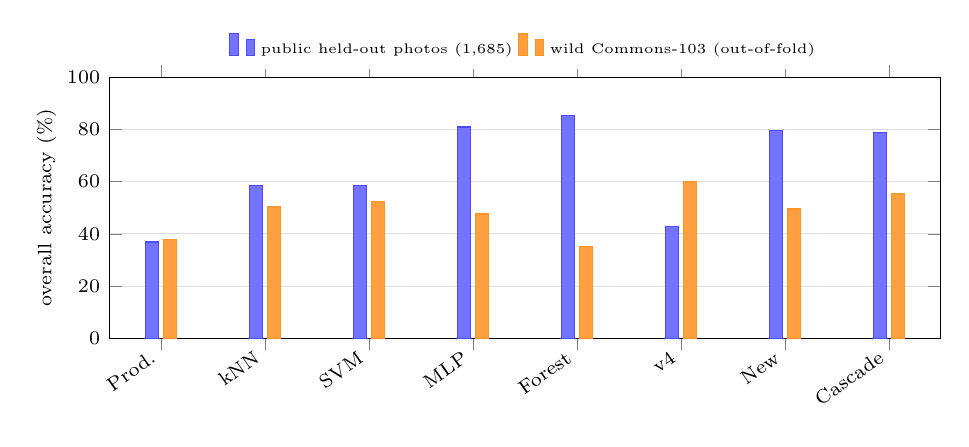
\begin{tikzpicture}
\begin{axis}[ybar,bar width=4.6pt,width=\columnwidth,height=4.9cm,ymin=0,ymax=100,ylabel={overall accuracy (\%)},ylabel style={font=\scriptsize,yshift=-3pt},
  symbolic x coords={Prod.,kNN,SVM,MLP,Forest,v4,New,Cascade},xtick=data,x tick label style={font=\scriptsize,rotate=35,anchor=east},y tick label style={font=\scriptsize},
  legend style={font=\tiny,at={(0.5,1.03)},anchor=south,legend columns=2,draw=none},enlarge x limits=0.07,ymajorgrids,grid style={gray!25}]
\addplot[fill=blue!55,draw=blue!70] coordinates {(Prod.,36.9)(kNN,58.6)(SVM,58.4)(MLP,80.9)(Forest,85.3)(v4,42.9)(New,79.6)(Cascade,78.9)};
\addplot[fill=orange!75,draw=orange!85] coordinates {(Prod.,37.9)(kNN,50.5)(SVM,52.4)(MLP,47.6)(Forest,35.0)(v4,60.2)(New,49.5)(Cascade,55.3)};
\legend{public held-out photos (1{,}685),wild Commons-103 (out-of-fold)}
\end{axis}
\end{tikzpicture}

\caption{The ranking of methods changes with the photo source. Prod.: production before (rules); MLP: plain MLP; New: the new 3-head model alone; Cascade: ours. The forest leads on photos from the training sources and trails every learned method on wild photos.}
\label{fig:baseline}
\end{figure}
\textbf{Is the forest's lead a memorisation artefact?} We audited the public test set by the distance of each photo to its nearest \emph{training photo} in standardised angle space. Exact near-duplicates are rare: only 0.3\% of the 1{,}685 photos lie within 0.05 of a training photo and 4.4\% within 0.2. The forest's lead also holds in every distance quartile, including the farthest (Q4: 84.6\% against 77.0\% for the cascade, Table~\ref{tab:audit}), although every method is most accurate on photos closest to training photos.
\begin{table}[t]
\centering\footnotesize\setlength{\tabcolsep}{3.5pt}
\caption{Public held-out photos split into quartiles of distance to the nearest training photo (Q1 closest; 421--422 photos each): overall accuracy / false-alarm rate.}\label{tab:audit}
\begin{tabular}{@{}lrrrr@{}}
\toprule
Method & Q1 & Q2 & Q3 & Q4 \\ \midrule
Random forest & 93.1 / 16.2 & 82.7 / 19.6 & 81.0 / 9.2 & 84.6 / 1.7 \\
Plain MLP & 91.7 / 14.8 & 78.6 / 28.0 & 75.8 / 21.3 & 77.7 / 13.2 \\
New 3-head model alone & 90.5 / 16.2 & 77.9 / 32.9 & 74.1 / 25.2 & 75.8 / 16.3 \\
Cascade (ours) & 89.1 / 16.2 & 76.2 / 32.0 & 73.4 / 23.2 & 77.0 / 13.5 \\ \bottomrule
\end{tabular}
\end{table}
But the public held-out photos come from the same public datasets as the training photos, and on the wild Commons-103 set the ranking reverses: the forest is the weakest learned method (35.0\%), 13--25 points below the SVM (52.4\%), $k$-NN (50.5\%), plain MLP (47.6\%), the new network (49.5\%), the cascade (55.3\%) and $v4$ (60.2\%). We read this as: tree ensembles are the strongest method on photos like the training photos and the weakest on photos from another source, so no method is best on both. The cascade is within seven points of the best method on each set and keeps false alarms at 20.8\%; a tree--network ensemble is the obvious next experiment (Section~\ref{sec:limits}). We keep the 3-head network because the form and deviation heads, the 0.36\,M-parameter footprint and the better behaviour on wild photos matter for a coach that must run on any phone, and because it is the architecture of the project proposal; we do not claim it is the best frame-level namer on same-source photos.

\subsection{Held-out videos: the ST-GCN}
On three folds split by video (24 videos, 8{,}002 windows, 60 frames, stride 12), the final target-pose ST-GCN reaches \textbf{82.2\%} overall; because 60\% of the windows are transition/unknown this flatters it, so we also report \textbf{78.0\%} macro recall over the nine classes (76.9\% over the eight poses). Three poses clear the bar: child's pose (recall/precision $.74/.91$), corpse ($1.00/.85$) and downward dog ($.83/.77$); seated easy, tree and triangle are within about 0.07 of it (Fig.~\ref{fig:charts}b). The model is conservative: its misses go to transition/unknown instead of to another pose. Warrior~II and plank fail on precision ($.26$, $.18$): 158 transition windows are called Warrior~II and plank has only 30 windows. A less conservative threshold chosen without leakage (an offset on the transition logit, picked on two folds and applied to the third) leaves overall accuracy at 81.9\% and raises the passing poses to four (child, downward dog, triangle, seated easy; corpse then drops below the precision bar); no offset reaches six. We therefore claim three poses (four with the cross-fitted threshold) for the ST-GCN and keep the ``seven poses'' claim for the frame cascade.

\textbf{Old versus new.} Table~\ref{tab:stgcn} scores the sequence model that was live until this work against the new one on the same held-out windows. The 12 videos that arrived after the old models were trained make that subset clean for them. The old live model had macro recall of 18.8\% and answered (with confidence $\ge$ its gate) on 2.8\% of true-pose windows; the new model answers on 50.5\% at 88.1\% precision. The old model's named transitions are not measured here and the new model has a single generic transition class.
\begin{table}[t]
\centering\footnotesize
\caption{ST-GCN versions on the same held-out windows (12 videos new to the old models). ``Answered'' is the share of true-pose windows that reach the UI, with its precision.}\label{tab:stgcn}
\begin{tabular}{@{}lrrrr@{}}
\toprule
Model & Overall & Macro rec. & Passing & Answered / prec. \\ \midrule
Old original (Jul) & 67.3\% & 11.6\% & 0 & 0\% / -- \\
Old v2 & 67.8\% & 13.2\% & 0 & 1.8\% / 100\% \\
Old live & 68.9\% & 18.8\% & 0 & 2.8\% / 93.8\% \\
\textbf{New} & \textbf{76.9\%} & \textbf{82.1\%} & 2 & \textbf{50.5\% / 88.1\%} \\ \bottomrule
\end{tabular}
\end{table}

\textbf{The input-rate contract.} Fig.~\ref{fig:charts}c re-scores the same videos while subsampling every $k$-th frame. The new model keeps macro recall $0.82$ at the training rate (25\,fps) and $0.81$ at 12.5\,fps, then loses it ($0.51$ at 6.2\,fps, $0.41$ at 3.1\,fps, $0.39$ at 2.1\,fps); the old model, partly trained on slow windows, is better at slow rates but never exceeds $0.62$. This is why the web app now fills a time-based 25\,fps buffer. A server audit found the backend architecture and normalisation identical to the trainer's (maximum logit difference 0.0 on 64 windows) and the deployed endpoint matching a local run of the same weights on 40/40 and 60/60 windows, so the weakness of the old model was generalisation, not serving.
\textbf{What we have not yet measured.} We prepared a controlled comparison of the ST-GCN with an LSTM, a BiLSTM with multi-head attention (the recipe of PosePilot-style systems \cite{gadhvi2025posepilot}), a temporal CNN, a window-statistics MLP and an ST-GCN with the skeleton graph removed, all on the same folds and one training recipe (AdamW \cite{loshchilov2019adamw}, last epoch scored). It needs a GPU and could not be run because the weekly GPU quota was exhausted, so we make no claim here that the skeleton graph, or the ST-GCN over a recurrent model, is necessary; the evidence for the sequence model is its held-out performance and the comparison with the previous model above.

\subsection{Does the form score mean anything?}
No labelled good-versus-bad-form data exist for these poses, so we use a property test: on 648 held-out in-vocabulary photos, five trials each, one joint is broken by $45^\circ$. Table~\ref{tab:form} shows that the new gate's form score is high on good form (0.81) and drops in 85.0\% of trials, the best of the four models, while the deviation head's top-ranked joint is the broken one in only 12.4\% of trials (chance 6.7\%), which is why per-joint cues come from the angle bands.
\begin{table}[t]
\centering\footnotesize
\caption{Property test: one joint broken by $45^\circ$ (chance for ``points at the broken joint'' is 6.7\%).}\label{tab:form}
\begin{tabular}{@{}lrrr@{}}
\toprule
Model & Score, good form & Score drops & Top joint correct \\ \midrule
19 Jul original & 0.28 & 65.0\% & 8.1\% \\
3 Sep retrain & 0.67 & 74.9\% & 18.2\% \\
21 Sep $v4$ & 0.79 & 59.2\% & 6.7\% \\
\textbf{New} & \textbf{0.81} & \textbf{85.0\%} & 12.4\% \\ \bottomrule
\end{tabular}
\end{table}
The same test on the deployed endpoint with real MediaPipe angles from eight instructor clips gives a mean score of 0.94 while held, \textbf{0.25} with the left knee broken (a drop on every probe of every clip) but \textbf{0.92} with the left elbow broken: the score collapses for leg errors and is nearly blind to arm errors. Arm errors can only be caught, if at all, by the angle-band layer, and we do not claim whole-body form checking. (These clips are in the gate's training data, so this is a regression check of the deployed path, not a generalisation number.)

\subsection{End-to-end checks on a real phone and on recorded video}
\textbf{On-phone photo test.} With the production app running on the POCO M7 Pro through its CPU engine and a Wikimedia photo standing in for the camera, every answer of the live server was logged (Table~\ref{tab:phone}); a photo counts if the most frequent of three answers is the expected pose, and a pose passes at $\ge50\%$ of its photos. Eight of eleven poses pass; of the seven poses that passed the held-out benchmark, the six tested here all pass, while mountain, cobra and child's pose do not (mountain and cobra were already weak). These are still photos with labels taken from file titles, and the models trained on Commons photos, so some may have been seen: the test checks the on-phone path (engine, landmarks, server, label), not generalisation.
\begin{table}[t]
\centering\footnotesize
\caption{On-phone photo test (photos correct / tested). Two photos had no person found.}\label{tab:phone}
\begin{tabular}{@{}lcc@{\hspace{10pt}}lcc@{}}
\toprule
Pose & Correct & & Pose & Correct & \\ \midrule
Tree & 6/6 & \pass & Chair & 3/5 & \pass \\
Triangle & 5/5 & \pass & Corpse & 2/4 & \pass \\
Warrior II & 3/3 & \pass & Child's pose & 1/3 & miss \\
Downward dog & 4/4 & \pass & Cobra & 1/5 & miss \\
Seated easy & 4/5 & \pass & Mountain & 0/5 & miss \\
Plank & 3/4 & \pass & \multicolumn{3}{c}{\textbf{8 of 11 poses pass}} \\ \bottomrule
\end{tabular}
\end{table}

\textbf{Live replay on recorded video.} We replayed eight clips of held poses (six poses, real MediaPipe on instructor video) against the deployed Space as the app would call it: seven of eight clips scored $\ge0.81$ frame-level accuracy while the pose was held (call-weighted 88.4\%), with zero failed API calls. One Seated-easy clip failed (0.06: named upward dog throughout), so Seated easy is not reliable live. On three clips of continuous movement the system reported ``transitioning'' for 74\%, 92\% and 79\% of frames. All eight clips come from videos in the training data of the gate, so this is a plumbing check; the ST-GCN, deployed after, answered correctly on 100\% of calls for the four poses it knows and stayed ``transition/unknown'' for mountain and lunge, which are outside its vocabulary.

\subsection{The interface}
Fig.~\ref{fig:ui} shows the deployed interface on the phone in the three languages and both themes, in free and guided mode. The skeleton overlay uses the colours of Section~\ref{sec:models} and the score ring, ``For your body'' personal score and coaching cue update about every 1.5\,s.
\begin{figure*}[t]
\centering
\begin{subfigure}[t]{0.175\textwidth}\centering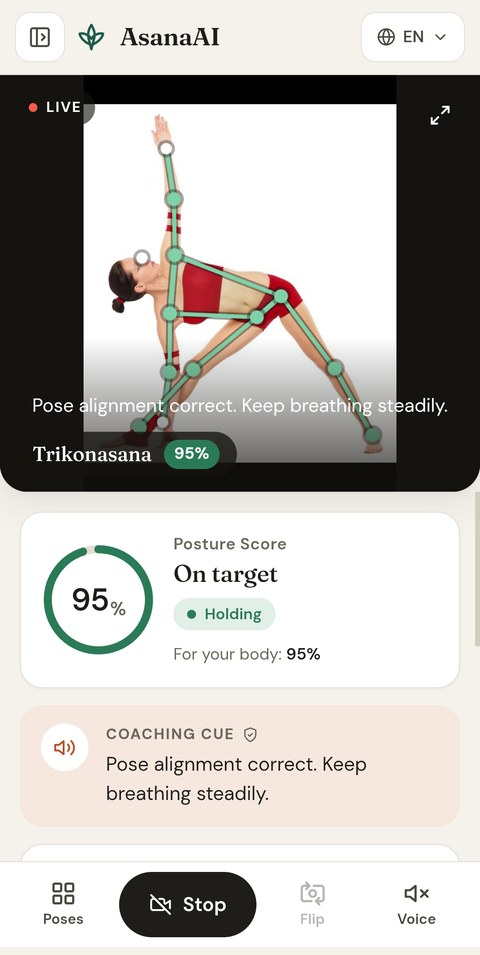
\includegraphics[width=\linewidth]{figures/ui_triangle_en.jpg}\caption{Free mode, English, light}\end{subfigure}\hfill
\begin{subfigure}[t]{0.175\textwidth}\centering
\includegraphics[width=\linewidth]{figures/ui_chair_hi.jpg}\caption{Hindi: 51\% form, amber}\end{subfigure}\hfill
\begin{subfigure}[t]{0.175\textwidth}\centering
\includegraphics[width=\linewidth]{figures/ui_warrior_bn_dark.jpg}\caption{Bengali, dark theme}\end{subfigure}\hfill
\begin{subfigure}[t]{0.175\textwidth}\centering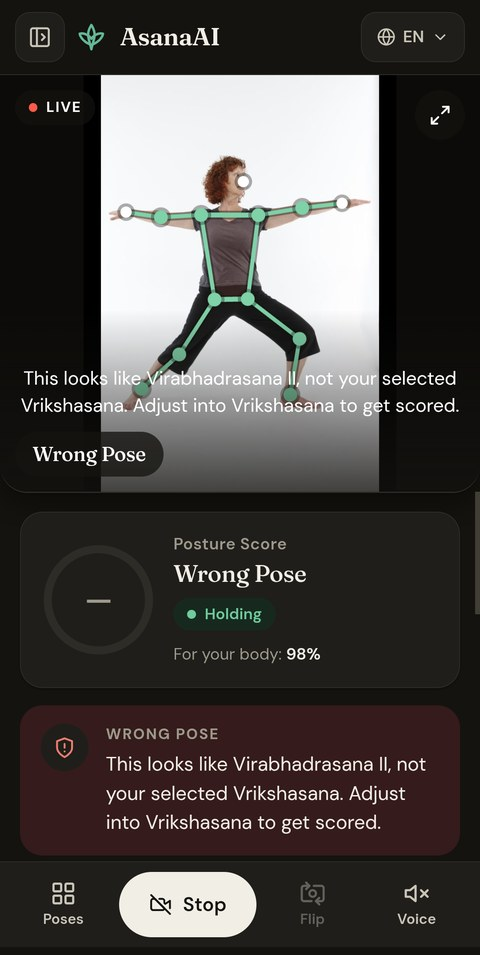
\includegraphics[width=\linewidth]{figures/ui_guided_wrong.jpg}\caption{Guided: wrong-pose card}\end{subfigure}\hfill
\begin{subfigure}[t]{0.175\textwidth}\centering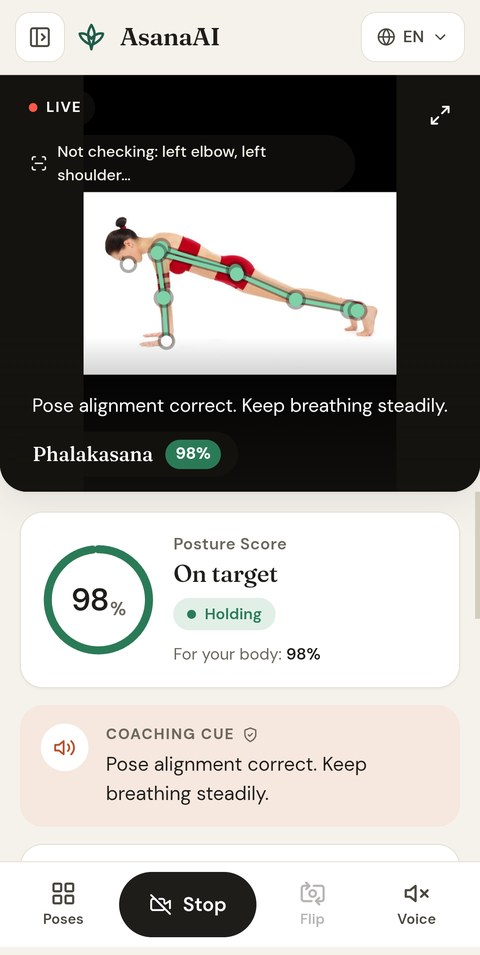
\includegraphics[width=\linewidth]{figures/ui_guided_plank.jpg}\caption{Guided: Plank, hidden joints}\end{subfigure}
\caption{The deployed interface on a POCO M7 Pro, a credited Wikimedia photo standing in for the camera (no live person): (a)~Trikonasana, 95\%; (b)~Utkatasana with the Hindi cue, 51\% in amber and a chip naming the joints not checked; (c)~Virabhadrasana~II in Bengali; (d)~guided mode with Vrikshasana selected while a Warrior~II photo is shown: the score is withheld and the app names the pose it sees; (e)~guided Plank (Phalakasana) with hidden joints named. Photos by Kennguru (a, b, e; CC BY 3.0), lululemon athletica (c, d; CC BY 2.0), via Wikimedia Commons.}
\label{fig:ui}
\end{figure*}
